\section{Accouting for sample heterogeneity}

\begin{frame}
  \frametitle{Handling scarcity and heterogeneity of data}

  \label{multi:scheme}
    
    \only<1>{Merge several experimental conditions}
    \only<2>{Inferring each graph \alert{independently} does not help}
    \only<3>{By \alert{pooling}  all the available data  (like we just
      have with Hess' data set)}
    \only<4->{By \alert{breaking} the separability}
  
  \vfill
  
  \begin{overlayarea}{\textwidth}{\textheight}
    
  \begin{tikzpicture}
    
    %% DATA 1
    \node at (-4.5,-0) {condition 1};
    \node[opacity=.75] (puce1)  at (-4.5,-1) {\pgfuseimage{ngs}};
    \node[opacity=.9]  (puce1b) at (-4.25,-1.25) {\pgfuseimage{ngs}};
    \node[opacity=.95] (puce1c) at (-4,-1.5) {\pgfuseimage{ngs}};
    
    %% DATA 2
    \node at (0,-0) {condition 2};
    \node[opacity=.75] (puce2)  at (0,-1) {\pgfuseimage{ngs}};
    \node[opacity=.9]  (puce2b) at (.25,-1.25) {\pgfuseimage{ngs}};
    \node[opacity=.95] (puce2c) at (.5,-1.5) {\pgfuseimage{ngs}};
    
    %% DATA 3
    \node at (4.5,-0) {condition 3};
    \node[opacity=.75] (puce3)  at (4.5,-1) {\pgfuseimage{ngs}};
    \node[opacity=.9]  (puce3b) at (4.75,-1.25) {\pgfuseimage{ngs}};
    \node[opacity=.95] (puce3c) at (5,-1.5) {\pgfuseimage{ngs}};
         
    %% independent inference
    \only<2,4-5>{
      \node (data1) at (-4,-2.75) {%
        \sf\scriptsize $(Y_1^{(1)},\dots,Y_{n_1}^{(1)})$
      };
      \node (data2) at (0.5,-2.75) {%
        \sf \scriptsize $(Y_1^{(2)},\dots,Y_{n_2}^{(2)})$
      };
      \node (data3) at (5,-2.75) {%
        \sf \scriptsize $(Y_1^{(3)},\dots,Y_{n_3}^{(3)})$
      };

      \path[->] (puce1c) edge (data1);
      \path[->] (puce2c) edge (data2);
      \path[->] (puce3c) edge (data3);

      \node[fill=red, text=white,single arrow, shape border rotate =270] 
      (inference1) at (-4,-3.25) {\sf \scriptsize inference}; 
      
      \node[fill=red, text=white,single arrow, shape border rotate =270] 
      (inference2) at (0.5,-3.25) {\sf \scriptsize inference}; 
      
      \node[fill=red, text=white,single arrow, shape border rotate =270] 
      (inference3) at (5,-3.25) {\sf \scriptsize inference}; 

   }
    \only<2>{
      %% GRAPH SETTINGS
      \tikzstyle{every edge}=[-,>=stealth',shorten >=1pt,auto,thin,draw]
      \tikzstyle{every node}=[fill=orange!70!white]
      \tikzstyle{every state}=[draw=none,text=white,scale=0.25, transform shape] 
      
      %% graph 1
      \node[state] (A1) at (-5.5,-6.0) {};
      \node[state] (A2) at (-5,-5.0) {};
      \node[state] (A3) at (-4.5,-6.0) {};
      \foreach \name/\angle/\text in {B1/234/G3, B2/162/G4, B4/18/G6, B3/90/G5, B5/-54/G7} {
        \node[state,xshift=-14cm,yshift=-21cm]     (\name)    at
        (\angle:.5cm) {}; }
 
      \path (A2) edge [bend left] (B3)
      (A2) edge [bend right] (A1) 
      (A3) edge [bend right] (A2)
      (A3) edge (B2) 
      (B1) edge [bend left] (B3)
      (A3) edge [bend right] (B3);
      
      \path (B1) edge [bend right] (A1);
      \foreach \from/\to in {1/2,2/3}{
        \path (B\from) edge [bend left] (B\to);
      }
      
      %% graph 2
      \node[state] (A1) at (-1,-6.0) {};
      \node[state] (A2) at (-0.5,-5.0) {};
      \node[state] (A3) at (0,-6.0) {};
      \foreach \name/\angle/\text in {B1/234/G3, B2/162/G4, B4/18/G6, B3/90/G5, B5/-54/G7} {
        \node[state,xshift=4cm,yshift=-21cm]     (\name)    at
        (\angle:.5cm) {}; }
    
      \path % (A1) edge [bend right] (B5) 
      (A2) edge [bend left] (B3)
      (A2) edge [bend right] (A1) 
      (A1) edge  (A3);
      
      \path (B1) edge [bend right] (A1);
      \foreach \from/\to in {1/3,3/5,5/1}{
        \path (B\from) edge [bend left] (B\to);
      }
      
      %% graph 3
      \node[state] (A1) at (3,-6.0) {};
      \node[state] (A2) at (3.5,-5.0) {};
      \node[state] (A3) at (4,-6.0) {};
      \foreach \name/\angle/\text in {B1/234/G3, B2/162/G4, B4/18/G6, B3/90/G5, B5/-54/G7} {
        \node[state,xshift=20cm,yshift=-21cm]     (\name)    at
        (\angle:.5cm) {}; }
      
      \path (A3) edge [bend right] (A2)
      (A3) edge (B2);
      
      \path (B1) edge (B4);
      \foreach \from/\to in {1/2,4/5,5/1,2/4}{
        \path (B\from) edge [bend left] (B\to);
      }
    }

    %% pooled inference
    \only<3>{
      \node (pooled) at (0.5,-2.75) {%
        \sf \scriptsize $(Y_1,\dots,Y_{n})$, $n=n_1+n_2+n_3$.
      };

      \path[->] (puce1c) edge (pooled);
      \path[->] (puce3c) edge (pooled);
      \path[->] (puce2c) edge (pooled);

      %% GRAPH SETTINGS
      \tikzstyle{every edge}=[-,>=stealth',shorten >=1pt,auto,thin,draw]
      \tikzstyle{every node}=[fill=orange!70!white]
      \tikzstyle{every state}=[draw=none,text=white,scale=0.25, transform shape] 
      
      \node[state] (A1) at (-1,-6.0) {};
      \node[state] (A2) at (-0.5,-5.0) {};
      \node[state] (A3) at (0,-6.0) {};
      \foreach \name/\angle/\text in {B1/234/G3, B2/162/G4, B4/18/G6, B3/90/G5, B5/-54/G7} {
        \node[state,xshift=4cm,yshift=-21cm]     (\name)    at
        (\angle:.5cm) {}; }
    
      \path % (A1) edge [bend right] (B5) 
      (A2) edge [bend left] (B3)
      (A2) edge [bend right] (A1)
      (A1) edge  (A3)
      (A3) edge [bend right] (A2)
      (A3) edge (B2) 
      (A3) edge [bend right] (B3);
      
      \path (B1) edge [bend right] (A1);
      \foreach \from/\to in {1/3,3/5,5/1,1/2,4/5,2/4}{
        \path (B\from) edge [bend left] (B\to);
      }
            
      \node[fill=red, text=white,single arrow, shape border rotate =270] 
      (inference) at (0.5,-3.25) {\sf \scriptsize inference}; 
    }

    %% multitask inference
    \only<4-5>{

      \path[->] (data1.east) edge [color=red] (inference2.west);
      \path[->] (data1.east) edge [color=red, bend right=5,in=175] (inference3.west);
      \path[->] (data2.west) edge [color=red] (inference1.east);
      \path[->] (data2.east) edge [color=red] (inference3.west);
      \path[->] (data3.west) edge [color=red, bend left=5,in=185] (inference1.east);
      \path[->] (data3.west) edge [color=red] (inference2.east);
    }
    \only<4>{

      %% GRAPH SETTINGS
      \tikzstyle{every edge}=[-,>=stealth',shorten >=1pt,auto,thin,draw]
      \tikzstyle{every node}=[fill=orange!70!white]
      \tikzstyle{every state}=[draw=none,text=white,scale=0.25, transform shape] 
      
      %% graph 1
      \node[state] (A1) at (-5.5,-6.0) {};
      \node[state] (A2) at (-5,-5.0) {};
      \node[state] (A3) at (-4.5,-6.0) {};
      \foreach \name/\angle/\text in {B1/234/G3, B2/162/G4, B4/18/G6, B3/90/G5, B5/-54/G7} {
        \node[state,xshift=-14cm,yshift=-21cm]     (\name)    at
        (\angle:.5cm) {}; }
 
      \path (A2) edge [bend left] (B3)
      (A2) edge [bend right] (A1) 
      (A1) edge  (A3)
      (A3) edge [bend right] (A2)
      (A3) edge (B2) 
      (B1) edge [bend left] (B3);
      
      \path (B1) edge [bend right] (A1);
      \foreach \from/\to in {1/2,2/3,3/5}{
        \path (B\from) edge [bend left] (B\to);
      }
      
      %% graph 2
      \node[state] (A1) at (-1,-6.0) {};
      \node[state] (A2) at (-0.5,-5.0) {};
      \node[state] (A3) at (0,-6.0) {};
      \foreach \name/\angle/\text in {B1/234/G3, B2/162/G4, B4/18/G6, B3/90/G5, B5/-54/G7} {
        \node[state,xshift=4cm,yshift=-21cm]     (\name)    at
        (\angle:.5cm) {}; }
    
      \path % (A1) edge [bend right] (B5) 
      (A2) edge [bend left] (B3)
      (A2) edge [bend right] (A1)
      (A3) edge (B2)
      (A1) edge  (A3) ;
      
      \path (B1) edge [bend right] (A1);
      \foreach \from/\to in {1/2,2/3,1/3,3/5,5/1}{
        \path (B\from) edge [bend left] (B\to);
      }
      
      %% graph 3
      \node[state] (A1) at (3,-6.0) {};
      \node[state] (A2) at (3.5,-5.0) {};
      \node[state] (A3) at (4,-6.0) {};
      \foreach \name/\angle/\text in {B1/234/G3, B2/162/G4, B4/18/G6, B3/90/G5, B5/-54/G7} {
        \node[state,xshift=20cm,yshift=-21cm]     (\name)    at
        (\angle:.5cm) {}; }
      
      \path (A3) edge [bend right] (A2)
      (A2) edge [bend left] (B3)
      (A3) edge (B2)
      (A1) edge  (A3) ;
      
      \path (B1) edge [bend right] (A1);
      \foreach \from/\to in {1/2,2/3,3/5,5/1}{
        \path (B\from) edge [bend left] (B\to);
      }
      
      \node[fill=red, text=white,single arrow, shape border rotate =270] 
      (inference) at (-4,-3.25) {\sf \scriptsize inference}; 
      
      \node[fill=red, text=white,single arrow, shape border rotate =270] 
      (inference) at (0.5,-3.25) {\sf \scriptsize inference}; 
      
      \node[fill=red, text=white,single arrow, shape border rotate =270] 
      (inference) at (5,-3.25) {\sf \scriptsize inference};       
    }
  \end{tikzpicture}

  \begin{block}{Multiple inference of GGM}<5>
    \begin{equation*}
      \argmax_{\boldsymbol\Theta^{(c)}, c=1\dots,C} 
      \sum_{c=1}^C
      \ell( \boldsymbol\Theta^{(c)};
      \mathbf{S}^{(c)}) -
      \lambda \ \mathrm{pen}_{\ell_1}(\boldsymbol\Theta^{(c)}).
    \end{equation*}
  \end{block}

\end{overlayarea}

\end{frame}

\begin{frame}
  \frametitle{A multitask approach}
  \framesubtitle{Chiquet, Grandvalet, Ambroise, Statistics and Computing 2010/11}

  \begin{overlayarea}{\textwidth}{\textheight}
    
  \begin{block}{Break the separability}
    Joint the optimization problem by either modifying
    \begin{equation*}
      \argmax_{\boldsymbol\Theta^{(c)}, c=1\dots,C} 
      \sum_{c=1}^C
      \tilde{\ell}(                           \boldsymbol\Theta^{(c)};
      \only<2>{\alert{\tilde{\mathbf{S}}^{(c)}}}\only<1,3>{\tilde{\mathbf{S}}^{(c)}})
      - \lambda \ \alert<3>{\mathrm{pen}_{\ell_1}(\boldsymbol\Theta^{(c)})}.
    \end{equation*}
  \begin{enumerate}
  \item \alert<2>{the fitting term}
  \item \alert<3>{the regularization term}
  \end{enumerate}
  \end{block}
  
  \only<2>{
    \begin{block}{Intertwined-Lasso}
      \begin{itemize}
      \item       $\overline{\mathbf{S}}       =      \frac{1}{n}\sum_{t=1}^T
        n_t\mathbf{S}^{(t)}$ is the ``pooled-tasks'' covariance matrix.
      \item $\widetilde{\mathbf{S}}^{(t)} = \alpha \mathbf{S}^{(t)} +
        (1-\alpha)\overline{\mathbf{S}}$ is a mixture between specific and pooled
        covariance matrices.
      \end{itemize}    
    \end{block}
  }
  
  \only<3>{
    \begin{block}{Sparsity with grouping effect}
      \begin{itemize}
      \item Group-Lasso (Yuan and Lin 2006, Grandvalet and Canu, 1998),
      \item Cooperative-Lasso (Chiquet et al, AoAS, 2012),
      \end{itemize}
    \end{block}
  }
  \end{overlayarea}
  
\end{frame}

\begin{frame}
  \frametitle{Grouping effects induced}

  \centering
  \begin{small}
    \begin{tabular}{lc@{\hspace{.1cm}}cc}
      & Potential groups & \multicolumn{2}{c}{Group(s) induced by edges $(1,2)$} \\
      \rotatebox{90}{\hspace{1cm}Group-\textsc{Lasso}} & 
      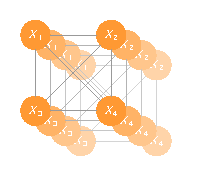
\includegraphics[width=.3\textwidth]{figures/grouping_grp_1} & 
      \multicolumn{2}{c}{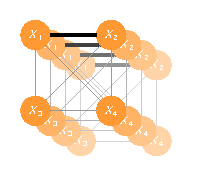
\includegraphics[width=.3\textwidth]{figures/grouping_grp_2}} \\
      \rotatebox{90}{\hspace{.35cm}Cooperative-\textsc{Lasso}} &
      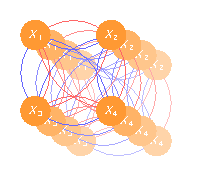
\includegraphics[width=.3\textwidth]{figures/grouping_coop_1} & 
      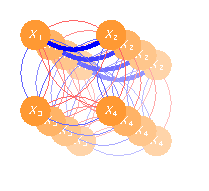
\includegraphics[width=.3\textwidth]{figures/grouping_coop_2} & 
      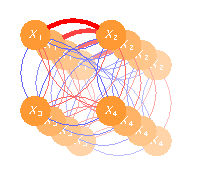
\includegraphics[width=.3\textwidth]{figures/grouping_coop_3} \\
    \end{tabular}
  \end{small}
\end{frame}


% \begin{frame}
%   \frametitle{Other grouping effects induced}
% 
%   \begin{beamerboxesrounded}[upper=sur:head,lower=sur:bloc,shadow=true]{Recent works}
%     \begin{itemize}
%     \item Use Fused-Lasso, sparse group-Lasso
%     \item  Adapted several  time  to the  \alert{Graphical Lasso  framework}
%       \begin{itemize}
%         \item\scriptsize See, e.g. D. Witten's team works.
%         \item\scriptsize The multitask/neighborhood selection's approach remains competitive.
%         \end{itemize}
%         \vspace{.5cm}
%       \item Mohan et al., 2014
%         \begin{itemize}
%         \item\scriptsize   Networks  differences   are  only   due  to
%           \alert{perturbations at the node level}.
%         \item\scriptsize For instance, a hub is encouraged to be shared across tasks.
%         \end{itemize}
%       \end{itemize}
%     \end{beamerboxesrounded}
% 
% \end{frame}

\begin{frame}
  \frametitle{Revisiting the Hess \textit{et al.} data set}
  
  \begin{figure}
    \centering
    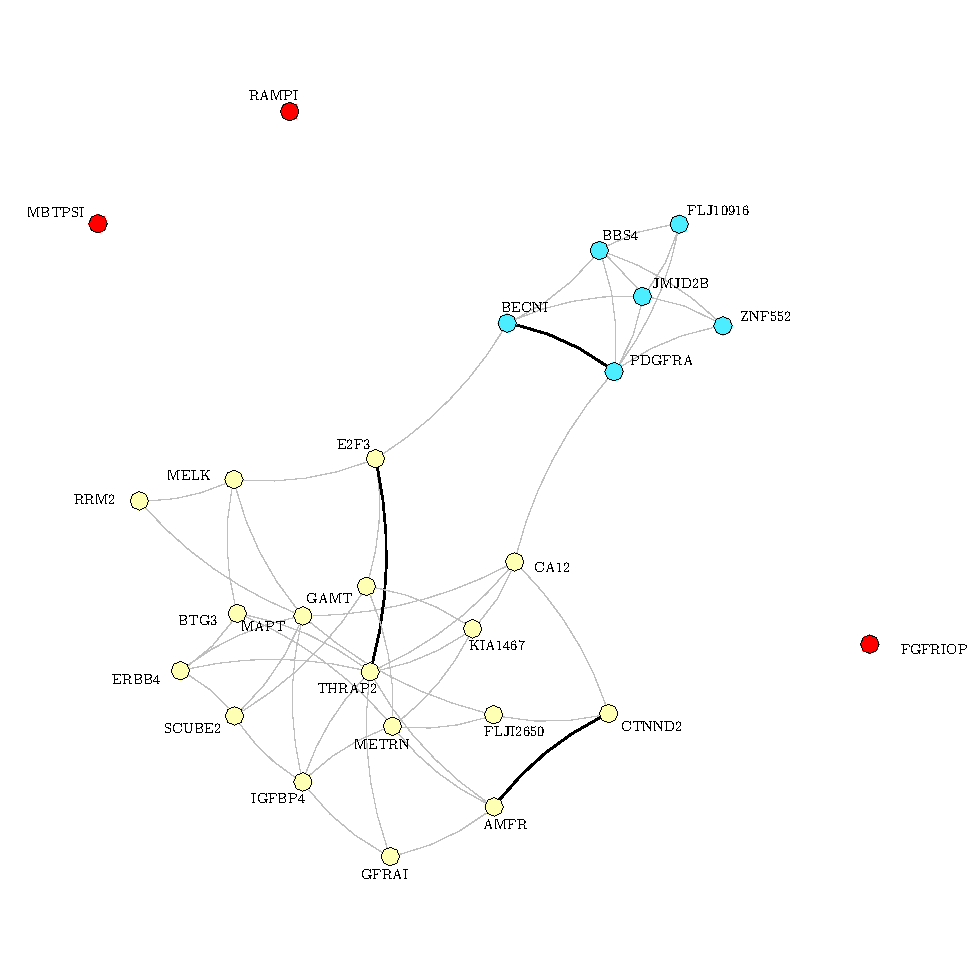
\includegraphics[width=.65\textwidth]{multi_breast}
    \caption{Cooperative-Lasso applied on the  two sets of patients
      (PCR/noPCR). Bold edges are different in the finally selection graph.} 
  \end{figure}

\end{frame}
